% ============================================================================
%  PROJECT & DATA OVERVIEW — Attachment for Data Request
%  Cloud-Native AI Operations Agent for CEM–CVM Intelligence
%  Souhayl Guenichi | ESPRIT | Huawei Tunisia | March 2026
% ============================================================================
\documentclass[12pt,a4paper]{article}

% -- Packages ----------------------------------------------------------------
\usepackage[utf8]{inputenc}
\usepackage[T1]{fontenc}
\usepackage[english]{babel}
\usepackage[top=2cm,bottom=2cm,left=2.2cm,right=2.2cm]{geometry}
\usepackage{lmodern}
\usepackage{microtype}
\usepackage{graphicx}
\usepackage[dvipsnames,svgnames,x11names]{xcolor}
\usepackage{tikz}
\usetikzlibrary{
  shapes.geometric,arrows.meta,positioning,fit,calc,
  backgrounds,shadows,decorations.markings
}
\usepackage{booktabs}
\usepackage{tabularx}
\usepackage{enumitem}
\usepackage{float}
\usepackage[font=small,labelfont=bf]{caption}
\usepackage[colorlinks=true,linkcolor=RoyalBlue,urlcolor=Crimson,
  pdfauthor={Souhayl Guenichi},
  pdftitle={AI Operations Agent — Project \& Data Overview}]{hyperref}
\usepackage{fancyhdr}
\pagestyle{fancy}\fancyhf{}
\fancyhead[L]{\small Project \& Data Overview}
\fancyhead[R]{\small\thepage}
\renewcommand{\headrulewidth}{0.4pt}
\setlength{\parskip}{4pt}
\setlength{\parindent}{0pt}

% -- Colors ------------------------------------------------------------------
\definecolor{huaweired}{HTML}{CF0A2C}
\definecolor{darkbg}{HTML}{2C3E50}
\definecolor{ossblue}{HTML}{2E86AB}
\definecolor{bssgreen}{HTML}{2ECC71}
\definecolor{aiviolet}{HTML}{8E44AD}
\definecolor{cvmorange}{HTML}{E67E22}
\definecolor{cemteal}{HTML}{1ABC9C}
\definecolor{datalake}{HTML}{3498DB}
\definecolor{actionred}{HTML}{E74C3C}

% -- TikZ Styles --------------------------------------------------------------
\tikzset{
  svc/.style={rectangle,rounded corners=4pt,minimum width=2.6cm,minimum height=0.9cm,
    draw=#1!70!black,fill=#1!15,text=black,font=\small\bfseries,
    drop shadow={shadow xshift=0.6pt,shadow yshift=-0.6pt,opacity=0.10},
    align=center,line width=0.6pt},
  svc/.default={ossblue},
  store/.style={cylinder,shape border rotate=90,aspect=0.25,
    minimum width=2cm,minimum height=1cm,
    draw=#1!70!black,fill=#1!12,text=black,font=\small\bfseries,
    align=center,line width=0.6pt},
  store/.default={datalake},
  ext/.style={rectangle,rounded corners=2pt,minimum width=2.2cm,minimum height=0.7cm,
    draw=gray!60,fill=gray!8,text=black,font=\small,dashed,align=center,line width=0.5pt},
  arr/.style={-{Stealth[length=5pt]},line width=0.7pt,#1},
  arr/.default={darkbg},
  lbl/.style={font=\scriptsize,fill=white,inner sep=1pt,text=darkbg},
}

% =============================================================================
\begin{document}

% -- HEADER -------------------------------------------------------------------
\begin{center}
{\large\textsc{ESPRIT} \quad$\cdot$\quad \textsc{Huawei Tunisia — Cloud IT}}\\[6pt]
\rule{0.8\linewidth}{0.6pt}\\[8pt]
{\LARGE\bfseries Cloud-Native AI Operations Agent\\[4pt]for CEM--CVM Intelligence}\\[6pt]
{\large Project Overview \& Required Datasets}\\[4pt]
\rule{0.8\linewidth}{0.6pt}\\[6pt]
{\small Souhayl Guenichi \quad|\quad End-of-Studies Project (PFE) \quad|\quad March 2026}
\end{center}

\vspace{0.4cm}

% =============================================================================
%  1. PROJECT OVERVIEW
% =============================================================================
\section*{1. Project Overview}

Telecom operators run two siloed systems: \textbf{CEM} (Customer Experience Management — Huawei SmartCare) monitors network quality through KPIs, while \textbf{CVM} (Customer Value Management) drives revenue decisions. When a cell degrades, the operations team detects the alarm, but no system automatically quantifies the business impact or triggers corrective action.

\textbf{Our platform is the missing intelligence layer between CEM and CVM.} It ingests network performance data (OSS) and subscriber/revenue data (BSS), applies AI models to detect anomalies, predict SLA risk, and correlate network degradation with business impact, then autonomously generates actionable recommendations for the CVM.

\begin{figure}[H]
\centering
\resizebox{\textwidth}{!}{%
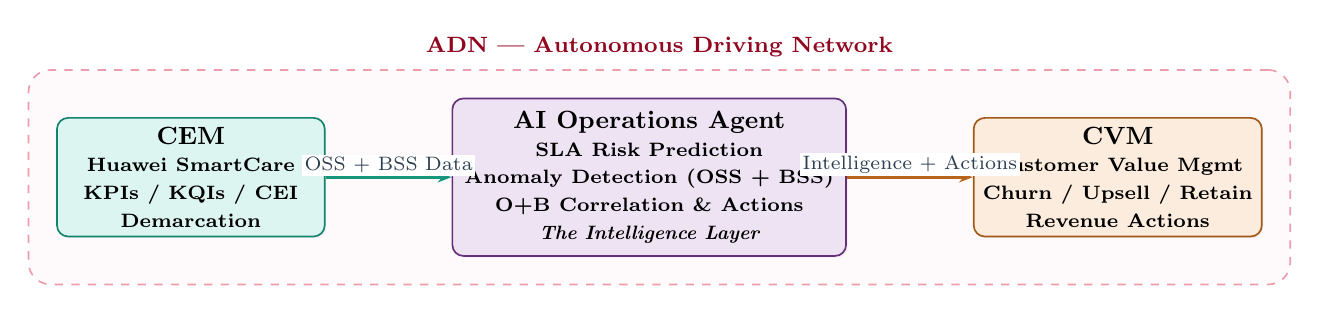
\begin{tikzpicture}[node distance=1.6cm]
  \node[svc=cemteal,minimum width=3.4cm,minimum height=1.5cm] (cem) {
    \textbf{CEM}\\[-1pt]{\scriptsize Huawei SmartCare}\\[-1pt]
    {\scriptsize KPIs / KQIs / CEI}\\[-1pt]{\scriptsize Demarcation}};
  \node[svc=aiviolet,minimum width=5cm,minimum height=2cm,right=of cem] (agent) {
    \textbf{AI Operations Agent}\\[-1pt]{\scriptsize SLA Risk Prediction}\\[-1pt]
    {\scriptsize Anomaly Detection (OSS + BSS)}\\[-1pt]
    {\scriptsize O+B Correlation \& Actions}\\[-1pt]
    {\scriptsize\bfseries\itshape The Intelligence Layer}};
  \node[svc=cvmorange,minimum width=3.4cm,minimum height=1.5cm,right=of agent] (cvm) {
    \textbf{CVM}\\[-1pt]{\scriptsize Customer Value Mgmt}\\[-1pt]
    {\scriptsize Churn / Upsell / Retain}\\[-1pt]{\scriptsize Revenue Actions}};
  \draw[arr=cemteal!80!black,line width=1pt] (cem) -- (agent)
    node[lbl,midway,above] {OSS + BSS Data};
  \draw[arr=cvmorange!80!black,line width=1pt] (agent) -- (cvm)
    node[lbl,midway,above] {Intelligence + Actions};
  \begin{scope}[on background layer]
    \node[fit=(cem)(agent)(cvm),inner sep=10pt,
      draw=huaweired!40,dashed,rounded corners=8pt,fill=huaweired!2,line width=0.6pt] (adn) {};
  \end{scope}
  \node[above=1pt of adn.north,font=\footnotesize\bfseries,text=huaweired!70!black] {
    ADN — Autonomous Driving Network};
\end{tikzpicture}}%
\caption{Industrial positioning: CEM $\to$ AI Agent $\to$ CVM.}
\end{figure}

\subsection*{What the Platform Delivers}

\begin{itemize}[nosep,leftmargin=1.2em]
  \item \textbf{SLA Risk Prediction} — a continuous risk score (0--1) per region, with the top contributing network KPIs explained.
  \item \textbf{Network Anomaly Detection} — per-cell anomaly alerts with severity scores, flagging degraded cells in real time.
  \item \textbf{Revenue Anomaly Detection} — per-subscriber anomaly detection for fraud, dormant SIMs, and churn spikes.
  \item \textbf{OSS--BSS Correlation} — statistical cross-domain analysis linking network degradation to revenue impact.
  \item \textbf{Autonomous Actions} — the agent generates recommendations (proactive alerts, churn prevention campaigns, upsell triggers) based on ML outputs and business rules.
\end{itemize}

% =============================================================================
%  2. SYSTEM ARCHITECTURE
% =============================================================================
\section*{2. System Architecture}

The platform runs as 5 containerised services, designed for local deployment (Docker Compose) with direct portability to Huawei Cloud Stack (HCS).

\begin{figure}[H]
\centering
\resizebox{\textwidth}{!}{%
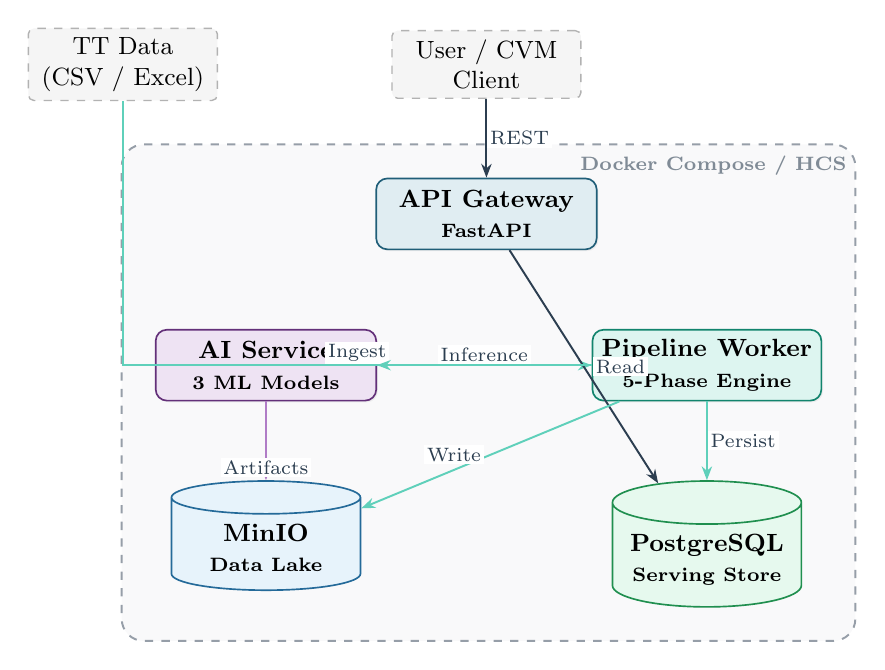
\begin{tikzpicture}[node distance=1cm and 1.6cm]
  \node[ext,minimum width=2.4cm] (user) {User / CVM\\Client};
  \node[ext,minimum width=2.4cm,left=2.2cm of user] (ttdata) {TT Data\\(CSV / Excel)};
  \node[svc=ossblue,below=1cm of user,minimum width=2.8cm] (apigw) {
    \textbf{API Gateway}\\{\scriptsize FastAPI}};
  \node[svc=aiviolet,below=of apigw,minimum width=2.8cm,xshift=-2.8cm] (ai) {
    \textbf{AI Service}\\{\scriptsize 3 ML Models}};
  \node[svc=cemteal,below=of apigw,minimum width=2.8cm,xshift=2.8cm] (worker) {
    \textbf{Pipeline Worker}\\{\scriptsize 5-Phase Engine}};
  \node[store=datalake,below=1cm of ai,minimum width=2.4cm] (minio) {
    \textbf{MinIO}\\{\scriptsize Data Lake}};
  \node[store=bssgreen,below=1cm of worker,minimum width=2.4cm] (pg) {
    \textbf{PostgreSQL}\\{\scriptsize Serving Store}};
  \begin{scope}[on background layer]
    \node[fit=(apigw)(ai)(worker)(minio)(pg),
      draw=darkbg!50,fill=darkbg!3,rounded corners=8pt,inner sep=12pt,
      line width=0.7pt,dashed] (docker) {};
  \end{scope}
  \node[below=1pt of docker.north east,anchor=north east,
    font=\scriptsize\bfseries,text=darkbg!60] {Docker Compose / HCS};
  \draw[arr] (user) -- (apigw) node[lbl,midway,right] {REST};
  \draw[arr=cemteal!70] (ttdata) |- (worker) node[lbl,pos=0.75,above] {Ingest};
  \draw[arr] (apigw) -- (pg) node[lbl,midway,right,xshift=3pt] {Read};
  \draw[arr=cemteal!70] (worker) -- (ai) node[lbl,midway,above] {Inference};
  \draw[arr=cemteal!70] (worker) -- (minio) node[lbl,midway,left,xshift=-2pt] {Write};
  \draw[arr=cemteal!70] (worker) -- (pg) node[lbl,midway,right] {Persist};
  \draw[arr=aiviolet!70] (ai) -- (minio) node[lbl,midway,below,yshift=-6pt] {Artifacts};
\end{tikzpicture}}%
\caption{Container architecture: 5 services with 3 ML models and a 3-layer data lake.}
\end{figure}

The AI service hosts three models: a \textbf{Gradient Boosting Regressor} for SLA risk prediction (supervised, 9 aggregated OSS features), and two \textbf{Isolation Forest} models for unsupervised anomaly detection on OSS and BSS data respectively. A statistical correlation engine (Pearson + Spearman) quantifies the relationship between network and business metrics. The Decision \& Action Engine evaluates all ML outputs against configurable business rules to generate typed, prioritised action recommendations.

% =============================================================================
%  3. REQUIRED DATASETS
% =============================================================================
\section*{3. Required Datasets}

The platform is fully operational on synthetic data. To achieve industrial validation and retrain models on real Tunisian operator behaviour, we require \textbf{two categories} of anonymised data from Tunisie Telecom.

\begin{figure}[H]
\centering
\resizebox{\textwidth}{!}{%
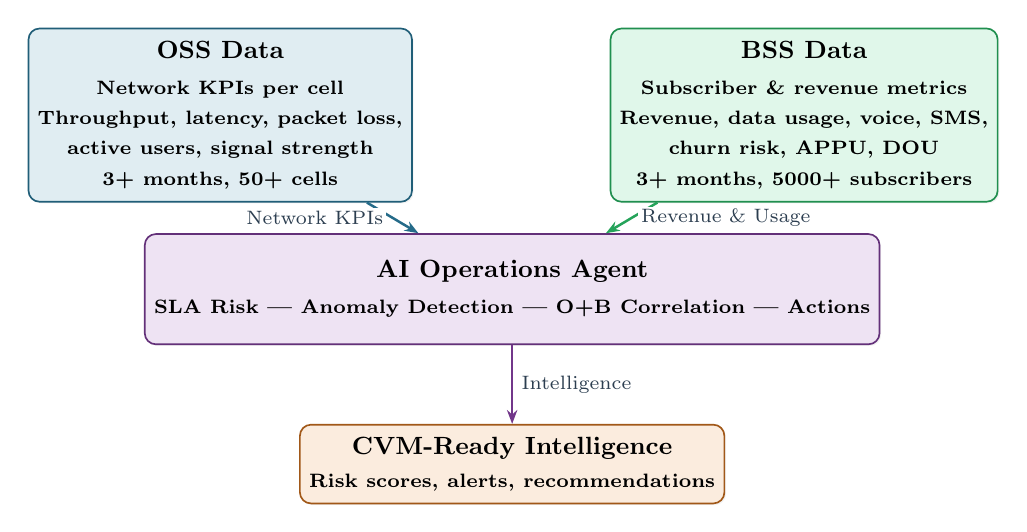
\begin{tikzpicture}[node distance=0.8cm and 2.5cm]
  \node[svc=ossblue,minimum width=4.5cm,minimum height=2.2cm] (oss) {
    \textbf{OSS Data}\\[2pt]
    {\scriptsize Network KPIs per cell}\\
    {\scriptsize Throughput, latency, packet loss,}\\
    {\scriptsize active users, signal strength}\\
    {\scriptsize 3+ months, 50+ cells}};
  \node[svc=bssgreen,minimum width=4.5cm,minimum height=2.2cm,right=2.5cm of oss] (bss) {
    \textbf{BSS Data}\\[2pt]
    {\scriptsize Subscriber \& revenue metrics}\\
    {\scriptsize Revenue, data usage, voice, SMS,}\\
    {\scriptsize churn risk, APPU, DOU}\\
    {\scriptsize 3+ months, 5000+ subscribers}};
  \node[svc=aiviolet,minimum width=5cm,minimum height=1.4cm,below=1.5cm of $(oss)!0.5!(bss)$] (agent) {
    \textbf{AI Operations Agent}\\[2pt]
    {\scriptsize SLA Risk | Anomaly Detection | O+B Correlation | Actions}};
  \node[svc=cvmorange,minimum width=4cm,minimum height=1cm,below=1cm of agent] (out) {
    \textbf{CVM-Ready Intelligence}\\[1pt]
    {\scriptsize Risk scores, alerts, recommendations}};
  \draw[arr=ossblue!80!black,line width=0.9pt] (oss) -- (agent)
    node[lbl,midway,left,xshift=-2pt] {Network KPIs};
  \draw[arr=bssgreen!80!black,line width=0.9pt] (bss) -- (agent)
    node[lbl,midway,right,xshift=2pt] {Revenue \& Usage};
  \draw[arr=aiviolet!80!black,line width=0.9pt] (agent) -- (out)
    node[lbl,midway,right,xshift=2pt] {Intelligence};
\end{tikzpicture}}%
\caption{The two data categories required and how they feed the AI Agent.}
\end{figure}

\subsection*{3.1\quad OSS Data — Network Performance KPIs}

Cell-level network performance measurements from the RAN / NOM layer. This data feeds the \textbf{SLA risk prediction model} and the \textbf{OSS anomaly detector}. The key metrics are radio and transport KPIs: downlink throughput, round-trip latency, packet loss rate, number of connected users, and reference signal power — all measured per cell over time.

\subsection*{3.2\quad BSS Data — Subscriber \& Revenue Metrics}

Per-subscriber business metrics from SmartCare BSS / CRM / billing systems. This data feeds the \textbf{revenue anomaly detector} and the \textbf{cross-domain correlation engine}. The key metrics are revenue per subscriber, data consumption, voice usage, SMS activity, churn indicators, and commercial plan information — reflecting the Tunisian market mix (${\sim}80\%$ prepaid / ${\sim}20\%$ postpaid).



\end{document}
